\documentclass[a4paper,11pt, hidelinks]{article}

\usepackage{listings}
\usepackage{lmodern}
\usepackage{amsmath,amssymb,amsthm,textcomp}
\usepackage[utf8]{inputenc}  
\usepackage[T1]{fontenc}  
\usepackage{graphicx}
\usepackage{float}
\usepackage{enumitem}
\usepackage{bbm}
\usepackage{caption}
\usepackage{hyperref}
\usepackage{cancel}
\usepackage{bigints}
\graphicspath{ {images/} }

\usepackage{geometry}
\geometry{total={210mm,297mm},
left=15mm,right=15mm,%
bindingoffset=0mm, top=5mm,bottom=20mm}

\usepackage{etoolbox}
\makeatletter
\preto{\@verbatim}{\topsep=0pt \partopsep=3pt }
\makeatother

\linespread{1}

\newcommand{\linia}{\rule{\linewidth}{0.5pt}}


% my own titles
\makeatletter
\renewcommand{\maketitle}{
\begin{center}
\vspace{2ex}
{\huge \textsc{\@title}}
\vspace{1ex}
\\
\linia\\
\@author 
\vspace{4ex}
\end{center}
}
\makeatother
%%%

% custom footers and headers
\usepackage{fancyhdr}
\pagestyle{fancy}
\lhead{}
\chead{}
\rhead{}

\cfoot{}
\rfoot{Page \thepage}
\renewcommand{\headrulewidth}{0pt}
\renewcommand{\footrulewidth}{0pt}
%
\DeclareMathOperator*{\argmax}{arg\,max}
\DeclareMathOperator*{\argmin}{arg\,min}
\DeclareMathOperator*{\var}{var}
\DeclareMathOperator*{\cov}{cov}

%%%----------%%%----------%%%----------%%%----------%%%

\begin{document}

\title{HW3}

\author{Gabriel ROMON}



\maketitle

\section*{Problem 7.5}

\begin{enumerate}[label=(\alph*)]
  \item Let us prove that $\frac 1{\int \frac{g(x)}{1-\rho(x)}dx}\frac{g(x)}{1-\rho(x)}$ is a stationary distribution for the Markov chain. It suffices to check the detailed balance condition (regardless of the normalizing constant). 
$$  \begin{aligned}
    \frac{g(x)}{1-\rho(x)} K(x,x') &=  \frac{g(x)}{1-\rho(x)} \left(\rho(x) \mathbbm 1_{x=x'}+(1-\rho(x))g(x') \right) 
    =  \frac{g(x')\rho(x')}{1-\rho(x')}\mathbbm 1_{x=x'} + g(x)g(x')  \\
    &= \frac{g(x')}{1-\rho(x')} \left(\rho(x') \mathbbm 1_{x'=x}+(1-\rho(x'))g(x) \right)\\
    &= \frac{g(x')}{1-\rho(x')} K(x',x)
  \end{aligned}$$

  \item Algorithm A.30 stems from the expression of $K(x,x')$: for a given $x^{(t)}$, $x^{(t+1)}$ is sampled from $g$ with probability $1-\rho(x^{(t)})$, and sampled from $\delta_{x^{(t)}}$ (that is to say $x^{(t+1)} = x^{(t)}$) with probability $\rho(x^{(t)})$.

  \item The Accept-Reject algorithm may be used to sample from the target distribution $f$ using $g$ as a proposal distribution, if an upper bound for $\displaystyle \frac fg \propto \frac{1}{1-\rho(x)}$ is known. On the contrary, algorithm A.30 does not require any such bound.\newline Besides, unlike Accept-Reject, this method does not discard any sample.
\end{enumerate}


\section*{Problem 7.6}

Assuming that $g\sim \mathcal Be(\alpha+1,1)$ and $\rho(x) = 1-x$, we get $\frac{g(x)}{1-\rho(x)} \propto \frac{x^{\alpha}}{x}=x^{\alpha-1}$, hence $f(x) = \alpha x^{\alpha-1}$.\newline \newline Samples of size $40.000$ were simulated for $\alpha \in \{0.3;0.9;1;1.1;2;5;10;20\}$ and $20.000$ points were kept after burn-in in each case. The results are displayed in Figure 1 and the code is in the Appendix.
\begin{figure}[H]
\centering
 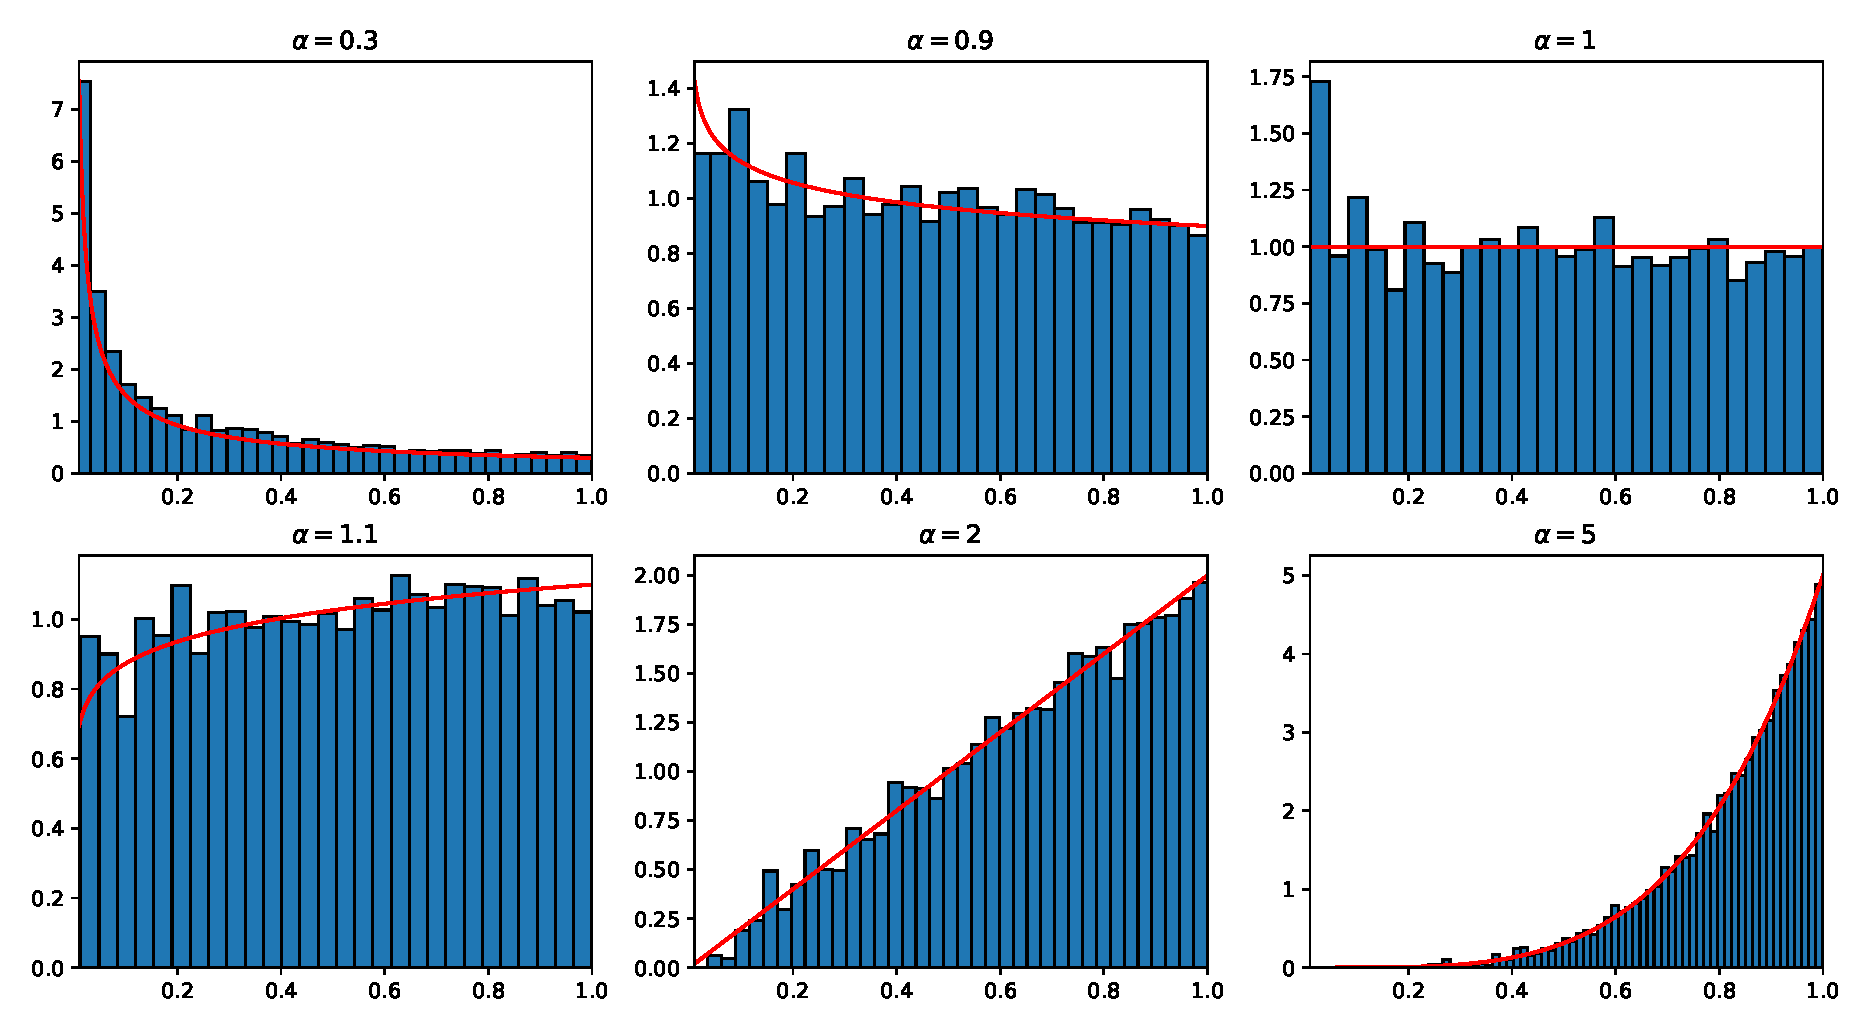
\includegraphics[scale=0.5]{plot.eps}  \\
\caption{Histograms of a sample of size $20.000$ obtained from the Repeat-Simulate algorithm, with the true density superimposed, for different values of $\alpha$}
\end{figure}

\noindent Note that for $\alpha=1$, $f$ is the uniform distribution over $[0,1]$. The results are satisfying since the histograms are a close approximation of the true density.


\section*{Problem 7.7}

$\bullet$ We have implemented the independent Metropolis-Hastings algorithm in the setting of Problem 7.6 (that is to say $g\sim \mathcal Be(\alpha+1,1)$ and $\rho(x) = 1-x$). The corresponding Python code is in the Appendix. With sample sizes and burn-in steps kept as before, we obtain similar results, as shown in Figure 2.

\begin{figure}[H]
\centering
 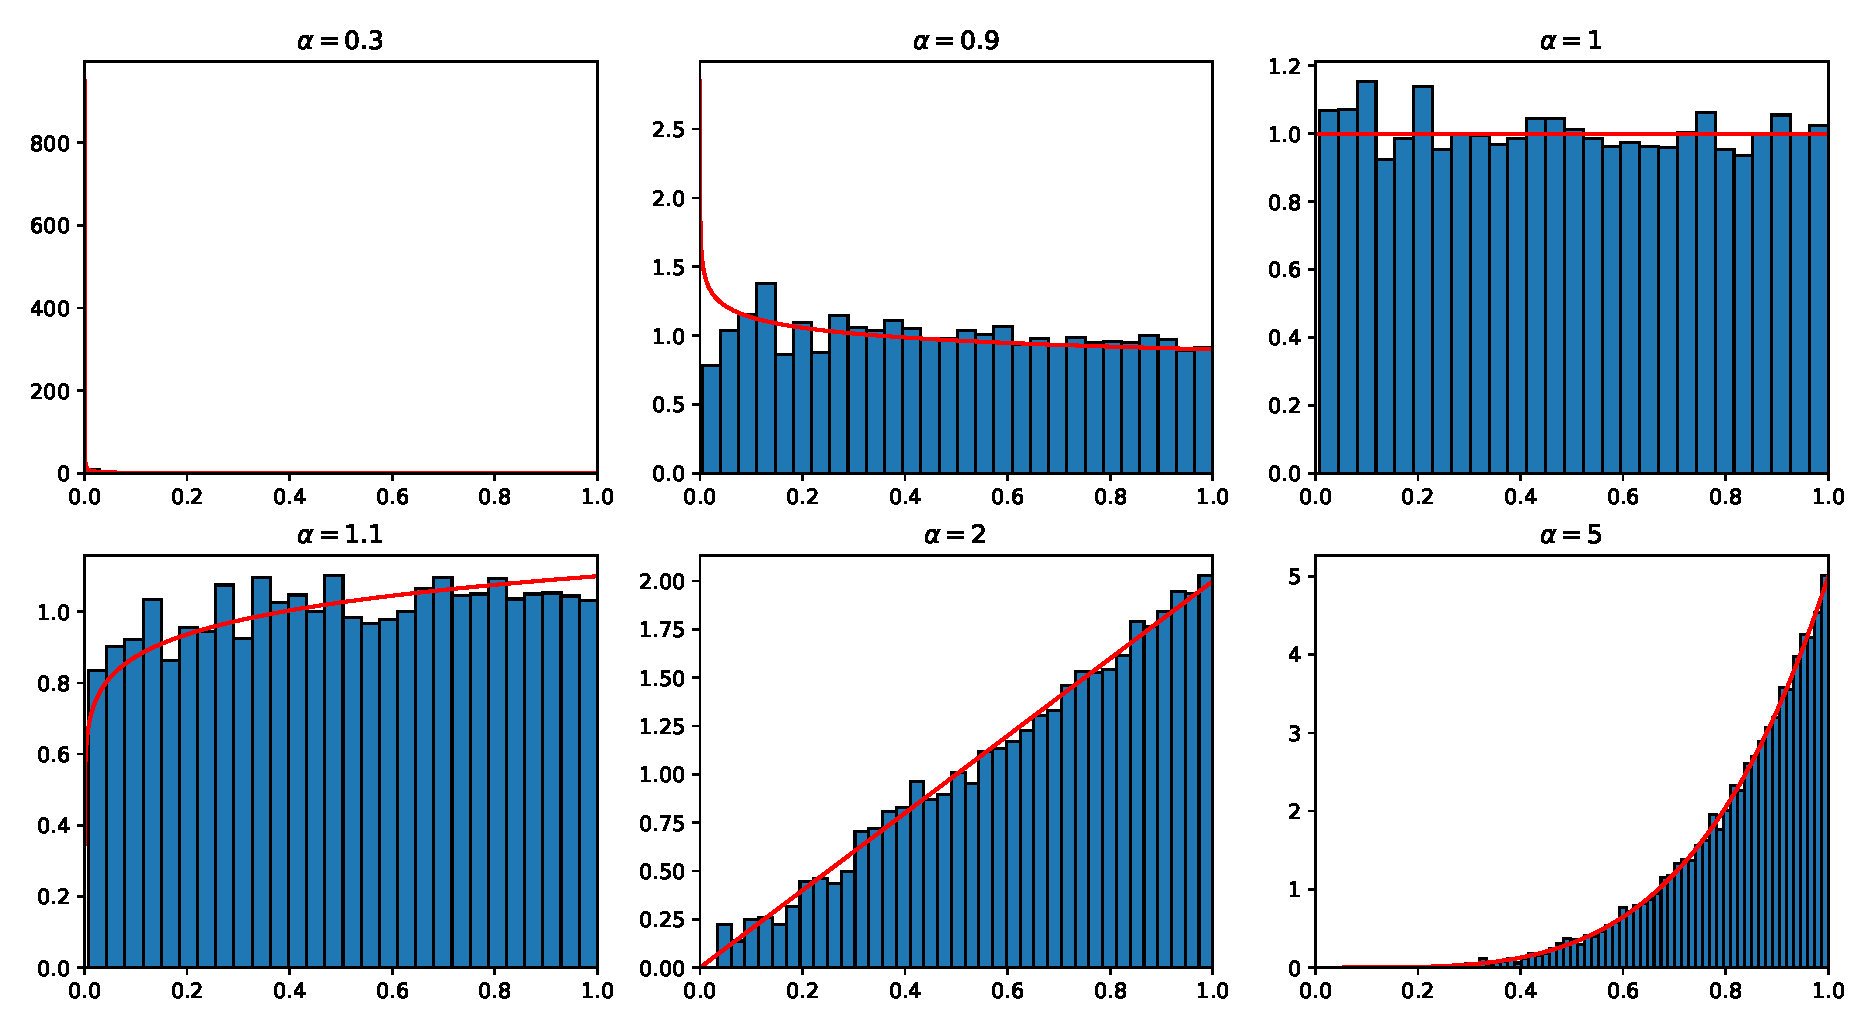
\includegraphics[scale=0.5]{plot2.eps}  \\
\caption{Histograms of a sample of size $20.000$ obtained from the independent Metropolis-Hastings algorithm, with the true density superimposed, for different values of $\alpha$}
\end{figure}

\hfill \newline 
\noindent $\bullet$  The methods can be compared in a more quantitative way by assessing how the respective samples perform on integral estimation. We chose to estimate the mean of $f$, which is $\displaystyle E_f(X) = \int_0^1 x f(x) dx = \frac{\alpha}{1+\alpha}$.\newline
Given a sample $x^{(1)},\ldots, x^{(T)}$ a natural estimator in this case is the sample mean $\delta := \frac 1T \sum_{i=1}^T x^{(i)}$.\newline
\newline
We compared the performance (in terms of computation time and variance) of this estimator, based on samples from the Repeat-Simulate algorithm, the independent Metropolis-Hastings algorithm and its Rao-Blackwellized counterpart. This last sampling method makes use of all the samples drawn from $g$ to reduce the variance, whereas the usual version rejects some of them. The expression for the Rao-Blackwellized estimator can be found in Theorem 7.19 in the book, and \textbf{we have provided a rigorous derivation below in Problem 7.31}. \newline \newline
We report computation times averaged over $7$ runs in Table 1, for a sample size of $20.000$. The Repeat-Simulate algorithm is quickest, although the independent Metropolis-Hastings is not far behind. The latter is slower because it has to sample from $g$ at every iteration. The Rao-Blackwellized version is significantly slower. Even though we optimized the code by making it as vectorized as possible and used a static compiler to speed up \verb!for! loops, the computations of the auxiliary variables $\zeta$ and $\tau$ require $O(T^2)$ multiplications, hence a much longer runtime.

\begin{figure}[H]
\centering
\begin{tabular}{|c|c|c|} \hline
Repeat-Simulate &  Independent Metropolis & Rao-Blackwellized \\ \hline
\begin{tabular}{c} $1.74\,\text{s} \pm 41.9 \,\text{ms}$
\end{tabular} &
\begin{tabular}{c} $2.41 \,\text{s} \pm 76.3 \,\text{ms}$
\end{tabular} &
\begin{tabular}{c} $27.5 \,\text{s} \pm 1.15 \,\text{s}$
\end{tabular}  \\ \hline
\end{tabular}
\captionof{table}{Time elapsed for estimation of the integral when using samples of size $20.000$ and $\alpha=5$. Times are averaged over $7$ runs. }
\end{figure}

\noindent Regarding variance, for each $\alpha\in \{0.5; 0.9; 1; 1.1; 5\}$ we sample $20.000$ points using each algorithm, perform a burn-in of $1000$, and collect the values of the mean squared error $\left(\delta - \frac{\alpha}{1+\alpha}\right)^2$. We repeat this experiment $100$ times and average the values we found to get an estimate of the variance. The results in Table 2 show that for any $\alpha$, the Rao-Blackwellized estimator performs best, and the variance reduction gets stronger as $\alpha$ grows: even though it is on par with the classic version when $\alpha=0.5$, its variance is $10$ times smaller when $\alpha = 5$. Besides, vanilla Independent Metropolis-Hastings performs slightly better than the Repeat-Simulate algorithm.

\begin{figure}[H]
\centering
\begin{tabular}{|c||c|c|c|} \hline 
$\alpha$ & Repeat-Simulate &  Independent Metropolis & Rao-Blackwellized \\ \hline\hline
\begin{tabular}{c} $0.5$
\end{tabular} &
\begin{tabular}{c} $1.025 \cdot 10^{-3}$
\end{tabular} &
\begin{tabular}{c} $9.726 \cdot 10^{-4}$
\end{tabular} &
\begin{tabular}{c} $7.643 \cdot 10^{-4}$
\end{tabular}  \\ \hline
\begin{tabular}{c} $0.9$
\end{tabular} &
\begin{tabular}{c} $2.825 \cdot 10^{-4}$
\end{tabular} &
\begin{tabular}{c} $2.551\cdot 10^{-4}$
\end{tabular} &
\begin{tabular}{c} $1.017 \cdot 10^{-4}$
\end{tabular}  \\ \hline
\begin{tabular}{c} $1$
\end{tabular} &
\begin{tabular}{c} $2.398 \cdot 10^{-4}$
\end{tabular} &
\begin{tabular}{c} $1.706\cdot 10^{-4}$
\end{tabular} &
\begin{tabular}{c} $7.785 \cdot 10^{-5}$
\end{tabular}  \\ \hline
\begin{tabular}{c} $1.1$
\end{tabular} &
\begin{tabular}{c} $1.467 \cdot 10^{-4}$
\end{tabular} &
\begin{tabular}{c} $1.798\cdot 10^{-4}$
\end{tabular} &
\begin{tabular}{c} $5.099\cdot 10^{-5}$
\end{tabular}  \\ \hline
\begin{tabular}{c} $5$
\end{tabular} &
\begin{tabular}{c} $5.657 \cdot 10^{-4}$
\end{tabular} &
\begin{tabular}{c} $3.734\cdot 10^{-4}$
\end{tabular} &
\begin{tabular}{c} $2.672\cdot 10^{-5}$
\end{tabular}  \\ \hline

\end{tabular}
\captionof{table}{Estimated variance of the sample mean estimator. $\alpha =5$, sample size is $20.000$ with a burn-in of $1000$}
\end{figure}

\noindent To conclude, the Repeat-Simulate algorithm is simpler and less computationally intensive compared to Metropolis-Hastings and its extensions. However, it exhibits higher variance.


\section*{Problem 7.31}

Let us first restate some context surrounding the independent Metropolis-Hastings algorithm. We assume that $x^{(0)}=y_0$ where $y_0$ is sampled according to $f$ (which is not a strong assumption since the generated Markov chain has $f$ as its stationary distribution). We also assume that $y_1,\ldots,y_T$ and $u_1,\ldots,u_T$ are i.i.d samples respectively from $g$ and $\mathcal U([0,1])$. For $t\geq 1$, by definition of the algorithm,  \begin{align*}x^{(t)} &= y_t \mathbbm 1\left\{u_t \leq \min \left(\frac{f(y_t)g(x^{(t-1)})}{f(x^{(t-1)})g(y_t)},1 \right)\right\} + x^{(t-1)} \mathbbm 1\left\{u_t > \min \left(\frac{f(y_t)g(x^{(t-1)})}{f(x^{(t-1)})g(y_t)}, 1 \right)\right\}\\
&=: \phi(x^{(t-1)}, y_t, u_t) \tag{1}\label{eq:1}
\end{align*}
Note that the $y_t, u_t, x^{(t)}$ are \textbf{random variables}. They will be treated as such in all the conditionings below. To estimate $E_f(h(X))$, a natural estimator is the empirical mean $\delta^{MH}$ which rewrites as $$\begin{aligned}
    \delta^{MH} &= \frac 1{T+1} \sum_{t=0}^T h(x^{(t)})  = \frac 1{T+1} \sum_{t=0}^T h(x^{(t)}) \sum_{i=0}^t \mathbbm 1_{y_i =x^{(t)}} \\
    &= \frac 1{T+1} \sum_{i=0}^{T}h(y_i)\sum_{t=i}^T  \mathbbm 1_{y_i =x^{(t)}}\\
    &= \frac 1{T+1} \sum_{t=0}^{T}h(y_t)\sum_{i=t}^T  \mathbbm 1_{x^{(i)} =y_t}
\end{aligned}$$
where the last equality enforces the notations used in the book.\newline
The Rao-Blackwellized version of the estimator is defined by $\delta^{RB} = E(\delta^{MH}|y_0,\ldots,y_T)$ where all the $y_t$ are used in the conditional expectation. The previous form of $\delta^{MH}$ implies $$\delta^{RB} = \frac 1{T+1} \sum_{t=0}^{T}h(y_t)\sum_{i=t}^T  P(x^{(i)} =y_t|y_0,\ldots,y_T)$$ and the goal of this problem is to provide a computationally tractable expression for $P(x^{(i)} =y_t|y_0,\ldots,y_T)$.

\begin{enumerate}[label=(\alph*)]
    \item Since by construction $x^{(0)} =y_0$, we have $\tau_0 = P(x^{(0)} =y_0|y_0,\ldots,y_T) =1$. For $i\geq 1$, \begin{align*}
        \tau_i = P(x^{(i)} =y_i|y_0,\ldots,y_T) &= E(\mathbbm 1_{x^{(i)} =y_i} | y_0,\ldots,y_T)\\
        &= E(E(\mathbbm 1_{x^{(i)} =y_i} |x^{(i-1)},y_0,\ldots,y_T)| y_0,\ldots,y_T) \tag{2}\label{eq:2}\\
    \end{align*}
    where the last equality follows from the tower property.
    Using the function $\phi$ defined in \eqref{eq:1}, the inner expectation rewrites as $$E(\mathbbm 1_{x^{(i)} =y_i} |x^{(i-1)},y_0,\ldots,y_T) = E\left[\mathbbm 1 \left\{\phi(x^{(i-1)}, y_i, u_i) =y_i \right\} |x^{(i-1)},y_0,\ldots,y_T\right]$$
    Let $P_{u_i}(\cdot|x^{(i-1)},y_0,\ldots,y_T)$ denote the regular conditional distribution of $u_i$ given $(x^{(i-1)},y_0,\ldots,y_T)$. Then $$\begin{aligned}
    E\left[\mathbbm 1 \left\{\phi(x^{(i-1)}, y_i, u_i) =y_i \right\} |x^{(i-1)},y_0,\ldots,y_T\right] &= 
        \int \mathbbm 1 \left\{\phi(x^{(i-1)}, y_i, u) =y_i \right\} dP_{u_i}(u|x^{(i-1)},y_0,\ldots,y_T)
    \end{aligned}$$
    Since $u_i$ is independent of $(x^{(i-1)},y_0,\ldots,y_T)$, $P_{u_i}(\cdot|x^{(i-1)},y_0,\ldots,y_T)$ simply collapses into $P_{u_i}(\cdot)$ and we get $$\begin{aligned}
    E\left[\mathbbm 1 \left\{\phi(x^{(i-1)}, y_i, u_i) =y_i \right\} |x^{(i-1)},y_0,\ldots,y_T\right] &= 
        \int \mathbbm 1 \left\{\phi(x^{(i-1)}, y_i, u) =y_i \right\} dP_{u_i}(u)\\
        &= \int \mathbbm 1 \left\{u\leq \min \left(\frac{f(y_i)g(x^{(i-1)})}{f(x^{(i-1)})g(y_i)},1 \right) \right\} dP_{u_i}(u)\\
        &= \min \left(\frac{f(y_i)g(x^{(i-1)})}{f(x^{(i-1)})g(y_i)},1 \right)\\
    \end{aligned}$$
    Consequently, \eqref{eq:2} becomes \begin{align*}
        \tau_i &= E\left[ \min \left(\frac{f(y_i)g(x^{(i-1)})}{f(x^{(i-1)})g(y_i)},1 \right) \bigg| y_0,\ldots,y_T\right]\\
        &= \sum_{j=0}^{i-1} E\left[ \min \left(\frac{f(y_i)g(x^{(i-1)})}{f(x^{(i-1)})g(y_i)},1 \right) \mathbbm 1_{x^{(i-1)}=y_j}\bigg| y_0,\ldots,y_T\right]\\
        &= \sum_{j=0}^{i-1} E\left[ \min \left(\frac{f(y_i)g(y_j)}{f(y_j)g(y_i)},1 \right) \mathbbm 1_{x^{(i-1)}=y_j}\bigg| y_0,\ldots,y_T\right]\\
        &= \sum_{j=0}^{i-1} \min \left(\frac{f(y_i)g(y_j)}{f(y_j)g(y_i)},1 \right) E\left[ \mathbbm 1_{x^{(i-1)}=y_j}\bigg| y_0,\ldots,y_T\right]\\
        &= \sum_{j=0}^{i-1} \rho_{ji} P(x^{(i-1)}=y_j| y_0,\ldots,y_T) \tag{3}\label{eq:3}
    \end{align*}

    \item $P(x^{(i-1)}=y_j| y_0,\ldots,y_T)$ still needs to be rewritten in a more tractable form. If $j=i-1$, this turns into $\tau_{i-1}$, so we may suppose $j<i-1$.\newline
    Note that $P(x^{(i-1)}=y_j| y_0,\ldots,y_T) = E(E(\mathbbm 1_{x^{(i-1)}=y_j}|x^{(i-2)}, y_0,\ldots,y_T)|y_0,\ldots,y_T)$ and computing the inner expectation as before yields $$E(\mathbbm 1_{x^{(i-1)}=y_j}|x^{(i-2)}, y_0,\ldots,y_T) = \left[1-\min \left(\frac{f(y_{i-1})g(x^{(i-2)})}{f(x^{(i-2)})g(y_{i-1})},1 \right)\right]\mathbbm 1_{x^{(i-2)}=y_j}$$
    Thus \begin{align*}P(x^{(i-1)}=y_j| y_0,\ldots,y_T)  &= E\left[\left(1-\min \left(\frac{f(y_{i-1})g(y_j)}{f(y_j)g(y_{i-1})},1 \right)\right)\mathbbm 1_{x^{(i-2)}=y_j} \bigg| y_0,\ldots,y_T\right] \\
    &= (1-\rho_{j(i-1)}) P(x^{(i-2)}=y_j| y_0,\ldots,y_T) \\
    &= (1-\rho_{j(i-1)}) (1-\rho_{j(i-2)})P(x^{(i-3)}=y_j| y_0,\ldots,y_T) \\
    &= \prod_{t=j+1}^{i-1}(1-\rho_{jt}) P(x^{(j)}=y_j| y_0,\ldots,y_T)\\
    &= \zeta_{j(i-1)} \tau_j \tag{4}\label{eq:4}
    \end{align*}
    Note that it remains valid for $j=i-1$ if one adds $\forall i, \zeta_{ii}=1$, which we do.
    Plugging this in \eqref{eq:3} yields $$\tau_i = \sum_{j=0}^{i-1} \rho_{ji}\zeta_{j(i-1)} \tau_j$$
    Using \eqref{eq:4} with different indexes, we derive the final form of $\delta^{RB}$:
    $$\delta^{RB} = \frac 1{T+1} \sum_{t=0}^{T}h(y_t)\sum_{i=t}^T \zeta_{ti} \tau_t = \frac 1{T+1} \sum_{i=0}^{T}h(y_i)\tau_i\sum_{j=i}^T \zeta_{ij}$$ where the last equality enforces notations used in Theorem 7.19 of the book. Hence $\varphi_i = \tau_i\sum_{j=i}^T \zeta_{ij}$.
\end{enumerate}



\section*{Problem 9.11}
\begin{enumerate}[label=(\alph*)]
    \item The inner integral rewrites as $$\int L^*(\theta|y,z)k(z|\theta', y) dz  = \int \frac{L(\theta|y,z)}{\int L(\theta|y,z) d\theta}\frac{L(\theta'|y,z)}{ L(\theta'|y)}dz$$
    Hence $$\int \left[\int L^*(\theta|y,z)k(z|\theta', y) dz\right] L^*(\theta'|y)d\theta' = \int \int \frac{L(\theta|y,z)}{\int L(\theta|y,z) d\theta}\frac{L(\theta'|y,z)}{ L(\theta'|y)}dz \frac{L(\theta'|y)}{\int L(\theta|y)d\theta} d\theta'$$
    Since the integrand is non-negative, Tonelli's theorem allows to switch the order of integration: 
    $$\begin{aligned}
        \int \left[\int L^*(\theta|y,z)k(z|\theta', y) dz\right] L^*(\theta'|y)d\theta' &= \int \left[\int \frac{L(\theta'|y,z)}{ \cancel{L(\theta'|y)}} \cancel{L(\theta'|y)}d\theta'\right] \frac{L(\theta|y,z)}{\int L(\theta|y,z) d\theta} \frac{1}{\int L(\theta|y)d\theta}dz \\
        &= \int \cancel{\int L(\theta'|y,z) d\theta'} \frac{L(\theta|y,z)}{\cancel{\int L(\theta|y,z) d\theta}} \frac{1}{\int L(\theta|y)d\theta}dz\\
        &= \frac{1}{\int L(\theta|y)d\theta} \int L(\theta|y,z)dz \\
        &= \frac{1}{\int L(\theta|y)d\theta}  L(\theta|y)\\
        &= L(\theta^*|y)
    \end{aligned}$$
    \item Consider some fixed $y$ and let $g_1(\theta|z) := L^*(\theta| y,z)$ and  $g_2(z|\theta) := k(z|\theta, y)$. By the Hammersley-Clifford theorem, if a joint distribution $g(\cdot,\cdot|y)$ exists for these conditional distributions, then it must satisfy $$\begin{aligned}g(\theta, z|y)&=\frac{g_2(z|\theta)}{\int \frac{g_2(z|\theta)}{g_1(\theta|z)}dz} = \frac{L(\theta|y,z)}{ L(\theta|y)} \frac{1}{\int\left[ \frac{L(\theta|y,z)}{ L(\theta|y)} \frac{\int L(\theta|y,z) d\theta}{L(\theta|y,z)}\right] dz}\\
    &= \frac{ L(\theta|y,z)}{\int \int L(\theta|y,z) dz d\theta} = \frac{ L(\theta|y,z)}{\int  L(\theta|y) d\theta}
    \end{aligned}$$
    The marginal density of $\theta$ is therefore $$g(\theta|y) = \int g(\theta, z) dz = \int \frac{ L(\theta|y,z)}{\int  L(\theta|y) d\theta}dz  = \frac{ L(\theta|y)}{\int  L(\theta|y) d\theta}= L^*(\theta|y)$$
    By a property of Gibbs sampling, $\theta_{(j)}$ is a Markov chain with a stationary distribution that has density $g(\theta|y) = L^*(\theta|y)$. Therefore, for $j$ large enough, $\theta_{(j)}$ can be considered as sampled from $L^*(\theta|y)$.\newline \newline
    Using this sample, the normalized likelihood $L^*(\theta|y)$ may be estimated by histograms or more elaborate kernel methods. However, the unnormalized likelihood remains out of reach, but it is not damaging if one intends to perform maximum likelihood estimation afterwards.
\end{enumerate}


\newpage
\section*{Appendix}

\textbf{Package imports}
\begin{verbatim}
import numpy as np
import scipy as sc 
from numba import jit
from numpy.random import binomial
from scipy.stats import beta
import matplotlib.pyplot as plt   
\end{verbatim}

\subsection*{Problem 7.5}
\textbf{Sampling using the Repeat-Simulate algorithm}
\begin{verbatim}
def sample(n, alpha):
    x0 = 0.5
    samples = [x0]
    for _ in range(n):
        if binomial(1,samples[-1]):
            samples.append(beta.rvs(alpha+1, 1, size=1)[0])
        else:
            samples.append(samples[-1])
    return samples

f, axarr = plt.subplots(2, 3, figsize = (15,8))
alphas = [0.3,0.9,1,1.1,2,5]
for (ax, alpha) in zip(axarr.flatten(), alphas): 
    x = np.linspace(0.01, 1, 2000)
    pdf = alpha*x**(alpha-1)
    ax.plot(x, pdf, 'r')
    ax.hist(sample(40000, alpha)[20000:], bins='auto', color='C0', 
                   density=True, ec='black')
    ax.set_xlim(0.01,1)
    ax.set_title(r'$\alpha = $'+str(alpha))
plt.show()
\end{verbatim}

\subsection*{Problem 7.7}
\textbf{Sampling using the independent Metropolis-Hastings algorithm}
\begin{verbatim}
def sample_metropolis_numpy(n, alpha):
    x0 = 0.5
    samples = np.full((n+1,), x0)
    ys = np.full((n+1,), x0)
    x = x0
    for i in range(1, n+1):
        y = beta.rvs(alpha+1, 1, size=1)[0]
        ys[i] = y
        prob = min(1, y**(alpha-1) * x**(alpha)/(x**(alpha-1) * y**(alpha)))
        if binomial(1,prob):
            samples[i] = y
            x = y
        else:
            samples[i] = x
    return (ys, samples)

f, axarr = plt.subplots(2, 3, figsize = (15,8))
alphas = [0.3,0.9,1,1.1,2,5]
for (ax, alpha) in zip(axarr.flatten(), alphas): 
    x = np.linspace(0.00001, 1, 2000)
    pdf = alpha*x**(alpha-1)
    ax.plot(x, pdf, 'r')
    ax.hist(sample_metropolis_numpy(40000, alpha)[1][20000:], bins='auto', color='C0',
            density=True, ec='black')
    ax.set_xlim(0.00001,1)
    ax.set_title(r'$\alpha = $'+str(alpha))
plt.savefig('plot2.eps', bbox_inches='tight')
plt.show()
\end{verbatim}

\hfill\newline \newline
\textbf{Integral estimation}
\begin{verbatim}
@jit(nopython=True)
def comp_metropolis_acc_numba(ys, alpha): 
    n = len(ys)-1
    zeta = np.zeros((n+1,n+1))
    tau = np.zeros(n+1)
    phi = np.zeros(n+1)
    
    w = alpha/(1+alpha)*1/ys
    rho = np.minimum(np.outer(1/w,w), 1)
    np.fill_diagonal(zeta, 1)
    temp = 1-rho
    for i in range(n):
        zeta[i, i+1:] = np.cumprod(temp[i, i+1:])
    tau[0] = 1
    phi[0] = np.sum(zeta[0, 0:])
    for i in range(1,n+1):
        tau[i] = np.sum(tau[:i]*zeta[:i, i-1]*rho[:i, i])
        phi[i] = tau[i]*np.sum(zeta[i, i:])
    return np.mean(phi*ys)    

alpha = 5
%timeit np.mean(sample(20000, alpha))
%timeit np.mean(sample_metropolis_numpy(20000, alpha))
%timeit ys, _ = sample_metropolis_numpy(20000, alpha); comp_metropolis_acc_numba(ys, alpha)

for alpha in [0.5, 0.9, 1, 1.1, 5]:
    val_true = alpha/(1+alpha)
    val_alg1, val_metro, val_metro_acc = [], [], []
    for _ in range(100):
        val_alg1.append(np.mean(sample(10000, 5)[1000:]))
        val_metro.append(np.mean(sample_metropolis(10000, 5)[1000:]))
        ys, _ = sample_metropolis_numpy(10000, alpha)
        val_metro_acc.append(comp_metropolis_acc_numba(ys[1000:], alpha))
    val_alg1 = np.array(val_alg1)
    val_metro = np.array(val_metro)
    val_metro_acc = np.array(val_metro_acc)
    
    print('alpha=', alpha)
    print(np.mean((val_alg1-val_true)**2))
    print(np.mean((val_metro-val_true)**2))
    print(np.mean((val_metro_acc-val_true)**2))
\end{verbatim}


\end{document}